\documentclass[12pt, twoside]{article}
\usepackage[letterpaper, margin=1in, headsep=0.5in]{geometry}
\usepackage[english]{babel}
\usepackage[utf8]{inputenc}
\usepackage{amsmath}
\usepackage{amsfonts}
\usepackage{amssymb}
\usepackage{tikz}
%\usetikzlibrary{quotes, angles}

\usepackage{graphicx}
\usepackage{enumitem}
\usepackage{multicol}

\usepackage{fancyhdr}
\pagestyle{fancy}
\fancyhf{}
\renewcommand{\headrulewidth}{0pt} % disable the underline of the header

\fancyhead[RE]{\thepage}
\fancyhead[RO]{\thepage \\ Name: \hspace{3cm}}
\fancyhead[L]{BECA / Dr. Huson / Geometry\\* 4 December 2019}

\begin{document}
\subsubsection*{6.6 Do Now: Distance formula, perpendicular and parallel slopes}
  \begin{enumerate}

  \item Write down the slope perpendicular to the given slope.
  \begin{enumerate}
    \begin{multicols}{2}
    \item   $m= -\frac{3}{5} \hspace{1cm} m_{\perp} = $ \vspace{1cm}
    %\item   $m= -2 \hspace{1cm} m_{\perp} = $
    \item   $m= 0.75 \hspace{1cm} m_{\perp} = $ \vspace{1cm}
    %\item   $m= \frac{1}{2} \hspace{1cm} m_{\perp} = $
    \end{multicols}
  \end{enumerate} \vspace{1cm}

  
  \item The line $l$ has the equation $y=-\frac{1}{2} x+3$.
  \begin{enumerate}
    \item What is the slope of the line $k$, given $k \parallel l$?
    \vspace{1.3cm}
    \item What is the slope of the line $j$, given $j \perp l$?
    \vspace{1.3cm}
  \end{enumerate}
  
  %\item What is the slope of a line perpendicular to the line $y=\frac{3}{2}x+1$?  \vspace{1.5cm}
  \item What is the slope of a line parallel to the line $x-2y=1$?  \vspace{2cm}
 
 
    \item Find $XY$, $X(-1,-6)$ and $Y(11,-6)$. \hspace{0.5cm}
    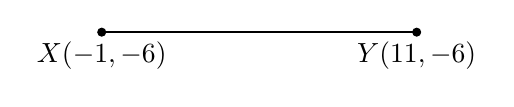
\begin{tikzpicture}[scale=1]
      \draw [thick] (0, 0)--(4,0);
      \draw [fill] (0,0) circle [radius=0.05] node[below]{$X(-1,-6)$};
      \draw [fill] (4,0) circle [radius=0.05] node[below]{$Y(11,-6)$};
    \end{tikzpicture} \vspace{1cm}

  \item Find $c$. \hspace{2cm}
    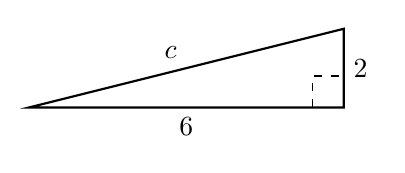
\begin{tikzpicture}[scale=1]
      \node at (2,0.5)[above left]{$c$};
      \node at (4,0.5)[right]{2};
      \node at (2,0)[below]{6};
      \draw [thick] (0, 0)--(4, 0)--(4, 1)--cycle;
      \draw [dashed] (4,0)++(-0.4,0)-- ++(0,0.4)-- +(0.4,0);
    \end{tikzpicture} \vspace{1.5cm}

  \item What is the length of $\overline{CD}$ if $C(3,1)$ and $D(7,-2)$?\\[0.5cm]
    Use $\displaystyle d=\sqrt{(x_2-x_1)^2+(y_2-y_1)^2}$

\newpage
  \item What is the midpoint of $\overline{HB}$, $H(80)$ and $B(120)$? \hspace{0.5cm}
  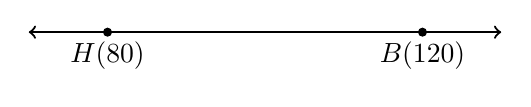
\begin{tikzpicture}[scale=1]
    \draw [thick, <->] (-1, 0)--(5,0);
    \draw [fill] (0,0) circle [radius=0.05] node[below]{$H(80)$};
    \draw [fill] (4,0) circle [radius=0.05] node[below]{$B(120)$};
  \end{tikzpicture} \vspace{1cm}

  \item Graph and label the two equations. Mark their intersection as an ordered pair.
    \begin{multicols}{2}
      $y = \frac{3}{2}x-9$ \\
      $2x+3y = 12$
    \end{multicols}     \vspace{2cm}
    Are the lines parallel, perpendicular, or neither? Justify your answer.
    \vspace{2cm}

    \begin{center} %4 quadrant regents grid w T-Chart
    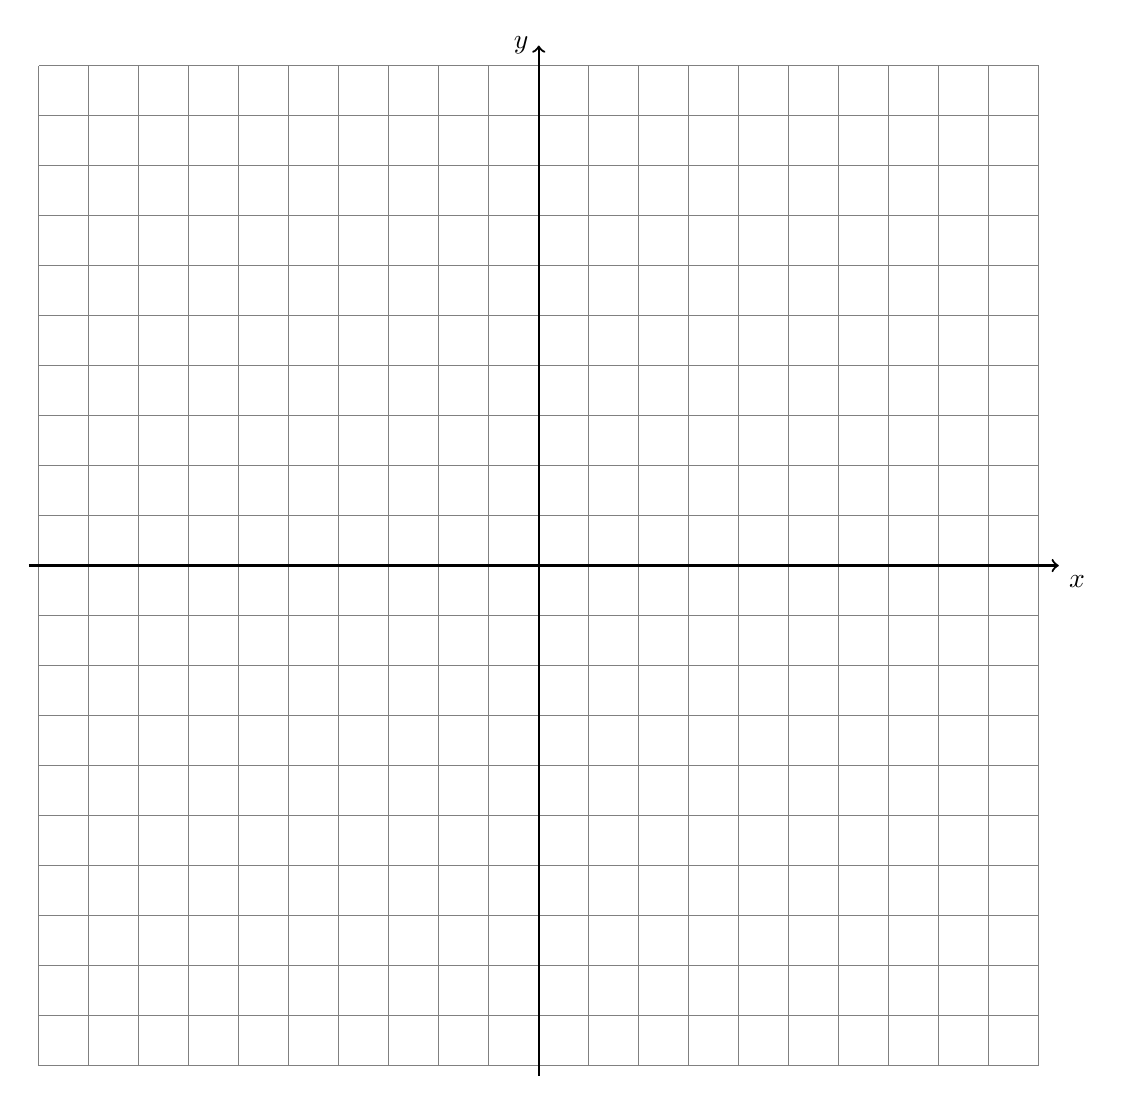
\begin{tikzpicture}[scale=.635]
      \draw [help lines] (-10,-10) grid (10,10);
      \draw [thick, ->] (-10.2,0) -- (10.4,0) node [below right] {$x$};
      \draw [thick, ->] (0,-10.2)--(0,10.4) node [left] {$y$};
    \end{tikzpicture}
    \end{center}

\end{enumerate}
\end{document}
